\documentclass[11pt,letterpaper]{article}

% ============================================================================
% PACKAGES
% ============================================================================
\usepackage[utf8]{inputenc}
\usepackage[T1]{fontenc}
\usepackage{helvet}
\renewcommand{\familydefault}{\sfdefault}
\usepackage[margin=0.85in, headheight=28pt]{geometry}
\usepackage{graphicx}
\usepackage{xcolor}
\usepackage{tikz}
\usepackage{tcolorbox}
\usepackage{booktabs}
\usepackage{enumitem}
\usepackage{hyperref}
\usepackage{fancyhdr}
\usepackage{titlesec}
\usepackage{multicol}
\usepackage{listings}
\usepackage{upquote}
\usepackage{amsmath,amssymb}
\usepackage{array}
\usepackage{longtable}

% Ragged-right paragraph columns to prevent word spacing issues
\newcolumntype{L}[1]{>{\raggedright\arraybackslash}p{#1}}

% Increase vertical spacing between table rows for readability
\renewcommand{\arraystretch}{1.2}

\usepackage{colortbl}
\usepackage{pifont}
\usepackage{setspace}
\usepackage{parskip}
\usepackage{caption}
\usepackage{tabularx}

\usetikzlibrary{shapes.geometric, arrows.meta, positioning, calc, decorations.pathreplacing, backgrounds, fit}

% ============================================================================
% COLOR DEFINITIONS - Hardware Security Theme (defense/cryptography)
% ============================================================================
% Primary: Steel blue - security, reliability, hardware
\definecolor{steelblue}{HTML}{2C3E7B}
\definecolor{lightblue}{HTML}{3498DB}
\definecolor{deepnavy}{HTML}{1A2744}
% Accent: Amber for warnings and security callouts
\definecolor{securityamber}{HTML}{E67E22}
\definecolor{alertred}{HTML}{C0392B}
% Domain colors
\definecolor{cryptogreen}{HTML}{27AE60}
\definecolor{sensorblue}{HTML}{2980B9}
\definecolor{fsmgold}{HTML}{F39C12}
\definecolor{wipecrimson}{HTML}{922B21}
% Neutrals
\definecolor{lightgray}{HTML}{F4F6F7}
\definecolor{medgray}{HTML}{BDC3C7}
\definecolor{softslate}{HTML}{5D6D7E}
\definecolor{textdark}{HTML}{1C2833}

% ============================================================================
% HYPERREF SETUP
% ============================================================================
\hypersetup{
  colorlinks=true,
  linkcolor=deepnavy,
  urlcolor=lightblue,
  pdftitle={Secure Terminal Briefcase: Tamper-Responsive Hardware Security System},
  pdfauthor={Hardware Systems Documentation}
}

% ============================================================================
% SPACING AND TYPOGRAPHY
% ============================================================================
\setstretch{1.15}
\setlength{\parskip}{0.5em}
\setlist{nosep, leftmargin=1.5em, itemsep=0.3em}

% ============================================================================
% PAGE STYLE - Circuit pattern (hardware/security theme)
% ============================================================================
\pagestyle{fancy}
\fancyhf{}
\fancyhead[L]{%
  \begin{tikzpicture}[baseline=-0.5ex]
    % Circuit-like pattern (hardware/engineering feel)
    \draw[lightblue, opacity=0.5, line width=0.6pt] (0,0.15) -- (0.3,0.15);
    \draw[lightblue, opacity=0.5, line width=0.6pt] (0.3,0.15) -- (0.3,0.3);
    \draw[lightblue, opacity=0.5, line width=0.6pt] (0.3,0.3) -- (0.6,0.3);
    \draw[lightblue, opacity=0.5, line width=0.6pt] (0.6,0.3) -- (0.6,0.0);
    \draw[lightblue, opacity=0.5, line width=0.6pt] (0.6,0.0) -- (0.9,0.0);
    \draw[lightblue, opacity=0.5, line width=0.6pt] (0.9,0.0) -- (0.9,0.15);
    \draw[lightblue, opacity=0.5, line width=0.6pt] (0.9,0.15) -- (1.2,0.15);
    \fill[steelblue, opacity=0.8] (0.3,0.15) circle (0.04);
    \fill[securityamber, opacity=0.8] (0.6,0.3) circle (0.04);
    \fill[steelblue, opacity=0.8] (0.9,0.15) circle (0.04);
  \end{tikzpicture}
  \hspace{0.4em}\textcolor{deepnavy}{\textsf{\small BRIEFCASE-2026-HW-002}}%
}
\fancyhead[R]{\textcolor{softslate}{\textsf{\thepage}}}
\fancyfoot[C]{\textcolor{softslate}{\footnotesize\textsf{Hardware Systems Documentation | Tamper-Responsive Security System}}}
\renewcommand{\headrulewidth}{0pt}
\renewcommand{\footrulewidth}{0pt}

\fancyheadoffset{0pt}
\setlength{\headheight}{32pt}

% ============================================================================
% SECTION FORMATTING
% ============================================================================
\titleformat{\section}
  {\normalfont\LARGE\bfseries\color{deepnavy}}
  {\thesection}{0.8em}{}[\vspace{-0.3em}{\color{lightblue}\rule{\textwidth}{1.5pt}\hspace{-\textwidth}\color{steelblue}\rule{3cm}{1.5pt}}]
\titleformat{\subsection}
  {\normalfont\Large\bfseries\color{deepnavy}}
  {\thesubsection}{0.6em}{}
\titleformat{\subsubsection}
  {\normalfont\large\color{softslate}\bfseries}
  {\thesubsubsection}{0.5em}{}

\titlespacing*{\section}{0pt}{3ex plus 1ex minus .2ex}{2ex plus .2ex}
\titlespacing*{\subsection}{0pt}{2.5ex plus 1ex minus .2ex}{1.5ex plus .2ex}

\setcounter{tocdepth}{3}

% ============================================================================
% TCOLORBOX ENVIRONMENTS
% ============================================================================
\tcbuselibrary{skins,breakable,hooks}

\newtcolorbox{keybox}[1][Key Design Principle]{
  enhanced, breakable,
  colback=steelblue!10, colframe=steelblue,
  colbacktitle=steelblue, coltitle=white,
  fonttitle=\bfseries\sffamily,
  title={\ding{72}\hspace{0.5em}#1},
  boxrule=0pt, leftrule=4pt, arc=0pt, outer arc=0pt,
  left=12pt, right=12pt, top=8pt, bottom=8pt
}

\newtcolorbox{securitybox}[1][Security]{
  enhanced, breakable,
  colback=securityamber!12, colframe=securityamber,
  colbacktitle=securityamber, coltitle=white,
  fonttitle=\bfseries\sffamily,
  title={\ding{73}\hspace{0.5em}#1},
  boxrule=0pt, leftrule=4pt, arc=0pt, outer arc=0pt,
  left=12pt, right=12pt, top=8pt, bottom=8pt
}

\newtcolorbox{hardwarebox}[1][Hardware Note]{
  enhanced, breakable,
  colback=sensorblue!10, colframe=sensorblue,
  colbacktitle=sensorblue, coltitle=white,
  fonttitle=\bfseries\sffamily,
  title={\ding{51}\hspace{0.5em}#1},
  boxrule=0pt, leftrule=4pt, arc=0pt, outer arc=0pt,
  left=12pt, right=12pt, top=8pt, bottom=8pt
}

\newtcolorbox{dangerbox}[1][Irreversible Operation]{
  enhanced, breakable,
  colback=alertred!10, colframe=alertred,
  colbacktitle=alertred, coltitle=white,
  fonttitle=\bfseries\sffamily,
  title={\ding{54}\hspace{0.5em}#1},
  boxrule=0pt, leftrule=4pt, arc=0pt, outer arc=0pt,
  left=12pt, right=12pt, top=8pt, bottom=8pt
}

% ============================================================================
% LISTINGS CONFIGURATION
% ============================================================================
\lstset{
  basicstyle=\small\ttfamily\color{textdark},
  backgroundcolor=\color{lightgray},
  frame=none,
  breaklines=true,
  breakatwhitespace=true,
  tabsize=2,
  showstringspaces=false,
  xleftmargin=1em,
  xrightmargin=1em,
  aboveskip=1em,
  belowskip=1em,
  numbers=none
}

\lstdefinelanguage{toml}{
  basicstyle=\small\ttfamily\color{textdark},
  comment=[l]{\#},
  commentstyle=\color{softslate}\itshape,
  string=[s]{"}{"},
  stringstyle=\color{steelblue},
}

% ============================================================================
% DOCUMENT
% ============================================================================
\begin{document}

% ============================================================================
% TITLE PAGE
% ============================================================================
\begin{titlepage}
\begin{tikzpicture}[remember picture, overlay]
  % Header band
  \fill[deepnavy] (current page.north west) rectangle ([yshift=-9cm]current page.north east);
  % Accent stripe
  \fill[steelblue] ([yshift=-9cm]current page.north west) rectangle ([yshift=-9.2cm]current page.north east);

  % Circuit pattern decoration
  \begin{scope}[shift={(current page.north west)}, xshift=1cm, yshift=-2cm, opacity=0.3]
    \foreach \x in {0,1,...,15} {
      \draw[lightblue, line width=0.4pt] (\x*1.2, 0) -- ++(0, -0.5) -- ++(0.6, 0) -- ++(0, 0.5);
    }
  \end{scope}
\end{tikzpicture}

\vspace*{1.5cm}

{\color{white}\sffamily
\begin{flushleft}
{\fontsize{14}{16}\selectfont HARDWARE SYSTEMS DOCUMENTATION}\\[0.3em]
{\fontsize{28}{32}\selectfont\bfseries Secure Terminal}\\[0.1em]
{\fontsize{28}{32}\selectfont\bfseries Briefcase}\\[0.2em]
{\fontsize{18}{22}\selectfont Tamper-Responsive Hardware Security System}\\[1.5em]
{\fontsize{11}{14}\selectfont System Design Document v1.0 --- February 2026}
\end{flushleft}
}

\vspace{2.5cm}

\begin{tcolorbox}[
  enhanced, width=0.92\textwidth,
  colback=lightgray, colframe=steelblue,
  boxrule=0pt, leftrule=4pt,
  left=15pt, right=15pt, top=12pt, bottom=12pt
]
\small\sffamily
\textbf{Platform}: Raspberry Pi 5 | Rust | systemd | Split-Privilege Services\\
\textbf{Sensors}: A3144 Hall Effect (primary) + BH1750 Light (secondary)\\
\textbf{Encryption}: LUKS2 FDE | AES-256-XTS | scrypt password hashing\\
\textbf{Recovery}: X25519 + ML-KEM-1024 (hybrid PQC) | ML-DSA-87 signatures\\
\textbf{Implementation}: \texttt{packages/tamper\_briefcase/}
\end{tcolorbox}

\vspace{1cm}

\begin{securitybox}[Defense-in-Depth Design]
This system provides physical security for a field-deployable agent terminal through layered defenses: dual-sensor tamper detection, password challenge with cryptographic verification, irreversible LUKS header destruction on failure, and quantum-safe encrypted recovery media. The split-privilege architecture ensures that a bug in any single component cannot trigger unintended data destruction.
\end{securitybox}

\vfill

{\small\color{softslate}\sffamily
Independent research --- not affiliated with any institution or committee\\
Published for defensive governance research and education\\
MIT License
}

\end{titlepage}

% ============================================================================
% TABLE OF CONTENTS
% ============================================================================
\tableofcontents
\newpage

% ============================================================================
% SECTION 1: SYSTEM ARCHITECTURE
% ============================================================================
\section{System Architecture}

The system secures a Raspberry Pi inside a hardened briefcase (Pelican 1490) with dual-sensor tamper detection, a 120-second password challenge on unauthorized opening, LUKS2 full-disk encryption with cryptographic wipe on authentication failure, and a hybrid classical+post-quantum encrypted recovery USB for reimaging.

\subsection{Physical Overview}

\begin{center}
\begin{tikzpicture}[font=\sffamily\small, scale=0.85, transform shape]
  % Outer briefcase
  \draw[line width=2pt, deepnavy, rounded corners=6pt] (0,0) rectangle (16,10);
  \node[font=\sffamily\footnotesize\color{softslate}] at (8,10.4) {Pelican 1490 Hard Case};

  % Lid region (top)
  \draw[line width=0.5pt, softslate, dashed] (0,6.5) -- (16,6.5);
  \node[font=\sffamily\footnotesize\color{softslate}, anchor=west] at (0.3,6.8) {--- LID ---};
  \node[font=\sffamily\footnotesize\color{softslate}, anchor=west] at (0.3,6.2) {--- BASE ---};

  % Magnet in lid
  \draw[fill=securityamber!30, rounded corners=2pt] (2,7.5) rectangle (4.5,8.5);
  \node[font=\sffamily\footnotesize\bfseries\color{securityamber}] at (3.25,8.3) {Neodymium};
  \node[font=\sffamily\footnotesize\color{softslate}] at (3.25,7.8) {Magnet};

  % Hall sensor (base, aligned under magnet)
  \draw[fill=sensorblue!20, rounded corners=2pt] (2,4.5) rectangle (4.5,5.8);
  \node[font=\sffamily\footnotesize\bfseries\color{sensorblue}] at (3.25,5.5) {Hall A3144};
  \node[font=\sffamily\scriptsize\color{softslate}] at (3.25,4.9) {GPIO 4};

  % Light sensor
  \draw[fill=fsmgold!20, rounded corners=2pt] (5.5,4.5) rectangle (8,5.8);
  \node[font=\sffamily\footnotesize\bfseries\color{fsmgold}] at (6.75,5.5) {BH1750};
  \node[font=\sffamily\scriptsize\color{softslate}] at (6.75,4.9) {I2C 0x23};

  % Alignment arrow
  \draw[-{Stealth[scale=0.8]}, dashed, securityamber, line width=0.8pt] (3.25,7.5) -- (3.25,5.8)
    node[midway, right=0.2cm, font=\sffamily\scriptsize\color{softslate}] {aligned};

  % Raspberry Pi
  \draw[fill=cryptogreen!15, rounded corners=3pt] (1,0.8) rectangle (8,3.8);
  \node[font=\sffamily\footnotesize\bfseries\color{cryptogreen}] at (4.5,3.4) {Raspberry Pi 5 (4GB+)};
  \node[font=\sffamily\scriptsize, align=center] at (4.5,2.3) {LUKS2 Root + Data\\tamper-sensor, tamper-gate\\tamper-challenge, tamper-recovery};

  % Sensor connections
  \draw[-{Stealth[scale=0.7]}, line width=0.8pt, sensorblue] (3.25,4.5) -- (3.25,3.8)
    node[midway, left=0.1cm, font=\sffamily\scriptsize] {GPIO};
  \draw[-{Stealth[scale=0.7]}, line width=0.8pt, fsmgold] (6.75,4.5) -- (6.75,3.8)
    node[midway, right=0.1cm, font=\sffamily\scriptsize] {I2C};

  % Power bank
  \draw[fill=steelblue!12, rounded corners=3pt] (9.5,0.8) rectangle (15,3.8);
  \node[font=\sffamily\footnotesize\bfseries\color{steelblue}] at (12.25,3.4) {USB-C Power Bank};
  \node[font=\sffamily\scriptsize, align=center] at (12.25,2.3) {10,000+ mAh\\Foam cradle (slides out)\\4--6 hr runtime};

  % USB-C connection
  \draw[-{Stealth[scale=0.7]}, line width=1pt, deepnavy] (8,2.3) -- (9.5,2.3)
    node[midway, above, font=\sffamily\scriptsize] {USB-C};

  % Recovery USB
  \draw[fill=wipecrimson!12, rounded corners=2pt] (9.5,4.5) rectangle (13.5,5.8);
  \node[font=\sffamily\footnotesize\bfseries\color{wipecrimson}] at (11.5,5.5) {Recovery USB};
  \node[font=\sffamily\scriptsize\color{softslate}] at (11.5,4.9) {PQC-wrapped keys};

  % Recovery connection
  \draw[-{Stealth[scale=0.7]}, line width=0.6pt, wipecrimson, dashed] (11.5,4.5) -- (8,3.2);
\end{tikzpicture}
\end{center}

\subsection{Split-Privilege Service Model}

The system splits into three systemd services enforcing least privilege. A bug in the sensor daemon cannot trigger a wipe; the wipe service requires an explicit trigger file created only by the gate after a confirmed challenge failure.

\begin{keybox}[Three-Service Architecture]
\begin{enumerate}
  \item \textbf{tamper-sensor} (unprivileged) --- Reads Hall + light sensors, emits JSON events + heartbeats via FIFO
  \item \textbf{tamper-gate} (root, restricted) --- Arming FSM, heartbeat watchdog, challenge dispatch, wipe authorization
  \item \textbf{tamper-wipe} (root, one-shot) --- luksSuspend + irreversible LUKS header destruction. Guarded by \texttt{ConditionPathExists}
\end{enumerate}
\end{keybox}

\begin{center}
\begin{tikzpicture}[node distance=2.8cm, font=\sffamily\small]
    \tikzstyle{service} = [rectangle, rounded corners=4pt, minimum width=12cm, minimum height=1.6cm,
      text centered, draw=textdark, line width=0.8pt, align=center]
    \tikzstyle{iface} = [font=\sffamily\scriptsize\color{softslate}, align=center]

    \node (sensor) [service, fill=sensorblue!12] {
      \textbf{tamper-sensor.service} (User: \texttt{tamper}, unprivileged)\\[-2pt]
      {\scriptsize Reads Hall + BH1750, emits LidOpened/LidClosed/LightAnomaly/Heartbeat via FIFO}};
    \node (gate) [service, below of=sensor, fill=fsmgold!12] {
      \textbf{tamper-gate.service} (Root, restricted write paths)\\[-2pt]
      {\scriptsize Arming FSM, heartbeat watchdog, spawns challenge subprocess, authorizes wipe}};
    \node (wipe) [service, below of=gate, fill=wipecrimson!12] {
      \textbf{tamper-wipe.service} (Root, one-shot)\\[-2pt]
      {\scriptsize luksSuspend $\rightarrow$ LUKS header destruction $\rightarrow$ poweroff. ConditionPathExists guard}};

    \draw [-{Stealth[scale=1.0]}, line width=1pt, deepnavy]
      (sensor.south) -- (gate.north) node[midway, right=0.4cm, iface] {Named FIFO\\JSON lines};
    \draw [-{Stealth[scale=1.0]}, line width=1pt, alertred]
      (gate.south) -- (wipe.north) node[midway, right=0.4cm, iface] {Trigger file\\+ systemctl start};
\end{tikzpicture}
\end{center}

This architecture provides:

\begin{itemize}
  \item \textbf{Least privilege}: The sensor daemon has zero write access to block devices or crypto subsystems.
  \item \textbf{Explicit gating}: The wipe can only execute when a trigger file exists, created only after a confirmed challenge failure.
  \item \textbf{Audit trail}: Each service logs independently. The wipe service activation is a distinct systemd event.
  \item \textbf{Reduced blast radius}: A bug in the sensor code cannot accidentally trigger a wipe.
\end{itemize}


% ============================================================================
% SECTION 2: DUAL-SENSOR TAMPER DETECTION
% ============================================================================
\newpage
\section{Dual-Sensor Tamper Detection}

\subsection{Why Two Sensors}

A light sensor alone is unreliable as a primary trigger. It suffers from seam leakage in bright environments, dark-current drift and temperature variation, and the ``briefcase moved under a lamp'' problem. Debouncing helps with noise but cannot distinguish ``lid opened'' from ``ambient conditions changed.''

The solution: a \textbf{Hall effect sensor as the authoritative lid-state indicator} and a \textbf{light sensor as secondary confirmation and anti-tamper evidence}.

\subsection{Sensor Roles}

\begin{longtable}{L{3cm} L{3.5cm} L{3.5cm} L{3.5cm}}
\toprule
\textbf{Sensor} & \textbf{Role} & \textbf{Failure Mode} & \textbf{Consequence} \\
\midrule
\endhead
Hall effect (A3144) & Primary: authoritative lid open/close detection & Magnet removed/shielded = permanent ``open'' reading & Triggers challenge (fail-safe) \\
BH1750 light sensor & Secondary: confirms physical exposure, detects bypass & Sensor covered or blinded & Hall still triggers independently \\
\bottomrule
\end{longtable}

\subsection{Decision Matrix}

\begin{center}
\begin{tikzpicture}[font=\sffamily\small]
  \matrix[matrix of nodes, row sep=0.2cm, column sep=0.3cm,
    nodes={minimum width=3.5cm, minimum height=0.9cm, anchor=center, rounded corners=2pt},
    row 1/.style={nodes={font=\sffamily\small\bfseries, fill=steelblue!15}},
    ] (m) {
    |[minimum width=3cm]| Hall State & |[minimum width=3cm]| Light Level & |[minimum width=5cm]| Result \\
    |[fill=cryptogreen!10]| CLOSED & |[fill=cryptogreen!10]| LOW & |[fill=cryptogreen!10]| Normal (armed, sleeping) \\
    |[fill=securityamber!15]| CLOSED & |[fill=securityamber!15]| HIGH & |[fill=securityamber!15]| Suspicious (log anomaly) \\
    |[fill=alertred!12]| OPEN & |[fill=alertred!12]| HIGH & |[fill=alertred!12]| Confirmed tamper \\
    |[fill=alertred!12]| OPEN & |[fill=alertred!12]| LOW & |[fill=alertred!12]| Tamper in dark (Hall is authoritative) \\
  };
\end{tikzpicture}
\end{center}

\begin{keybox}[Primary Sensor Authority]
Hall alone is sufficient to trigger a challenge. Light alone never triggers---it adds confidence and detects sensor-bypass scenarios. Consecutive light anomalies (configurable threshold, default 10) escalate to a forced challenge, detecting attempts to spoof the Hall sensor while the lid is physically open.
\end{keybox}

\subsection{Arming Delay}

Closing the briefcase does not instantly arm the system. The lid must remain continuously closed (Hall reading ``closed'') for a configurable delay (default 15 seconds) before transitioning from DISARMED to ARMED. This prevents false triggers while adjusting the latch or contents. Reopening during the arming window immediately returns to DISARMED.


% ============================================================================
% SECTION 3: HARDWARE DESIGN
% ============================================================================
\newpage
\section{Hardware Design}

All components are standard consumer and maker parts. Total estimated cost: \$280--\$400.

\subsection{Bill of Materials}

\subsubsection{Core Components}

\begin{longtable}{L{3.5cm} L{4cm} L{1cm} L{2cm} L{2cm}}
\toprule
\textbf{Component} & \textbf{Model} & \textbf{Qty} & \textbf{Est. Cost} & \textbf{Interface} \\
\midrule
\endhead
Raspberry Pi 5 & 4GB+ with PSU & 1 & \$60--80 & --- \\
MicroSD Card & Samsung PRO Endurance 128GB & 1 & \$20 & --- \\
Briefcase & Pelican 1490 Laptop Case & 1 & \$100--150 & --- \\
USB-C Power Bank & Anker 325 or similar (10,000mAh+) & 1 & \$25--35 & USB-C \\
USB-C Cable & 15cm right-angle & 1 & \$5 & USB-C \\
Recovery USB & IronKey or Samsung T7 Shield & 1 & \$50--80 & USB \\
\bottomrule
\end{longtable}

\subsubsection{Sensors}

\begin{longtable}{L{3.5cm} L{4cm} L{1cm} L{2cm} L{2cm}}
\toprule
\textbf{Component} & \textbf{Model} & \textbf{Qty} & \textbf{Est. Cost} & \textbf{Interface} \\
\midrule
\endhead
Hall Effect Sensor & A3144 (digital latch) & 1 & \$1--2 & GPIO 4 \\
Neodymium Magnet & 12mm N52 disc & 1 & \$2--3 & --- \\
Light Sensor & BH1750 (I2C breakout) & 1 & \$3--5 & I2C \\
Pull-up Resistor & 10k (for A3144) & 1 & \$0.10 & --- \\
\bottomrule
\end{longtable}

\subsection{Wiring}

\begin{hardwarebox}[Sensor Wiring]
\begin{lstlisting}
Hall Effect Sensor (A3144 -- digital latch)
-------------------------------------------
VCC  ----------> Pin 1  (3.3V)
GND  ----------> Pin 9  (GND)
OUT  ----------> Pin 7  (GPIO 4)
     +-- 10k pull-up to 3.3V

Magnet present -> OUT = LOW  (lid closed)
Magnet absent  -> OUT = HIGH (lid open)

BH1750 Light Sensor (I2C)
-------------------------
VCC  ----------> Pin 1  (3.3V)
GND  ----------> Pin 6  (GND)
SDA  ----------> Pin 3  (GPIO 2 / SDA1)
SCL  ----------> Pin 5  (GPIO 3 / SCL1)
ADDR ----------> GND    (sets I2C address to 0x23)
\end{lstlisting}
\end{hardwarebox}

\subsection{Physical Placement}

Mount the Hall sensor on the base of the briefcase near the latch mechanism. Epoxy a small neodymium disc magnet to the corresponding spot on the lid interior. When closed, the magnet sits directly above the Hall sensor (within $\sim$10mm). The BH1750 mounts nearby, oriented upward toward the lid seam---the first entry point for light.

\begin{securitybox}[Alignment is Critical]
The A3144 needs the magnet within $\sim$10mm when closed. Test alignment before permanently mounting---use blu-tack first, mark positions, then epoxy. Line the briefcase seam with adhesive foam weatherstripping for light sealing (aim for $<$1 lux when sealed).
\end{securitybox}


% ============================================================================
% SECTION 4: SOFTWARE ARCHITECTURE
% ============================================================================
\newpage
\section{Software Architecture}

\subsection{Crate Structure}

All application code is in Rust, organized as a Cargo workspace:

\begin{longtable}{L{3cm} L{3cm} L{7cm}}
\toprule
\textbf{Crate} & \textbf{Binary} & \textbf{Role} \\
\midrule
\endhead
\texttt{tamper-common} & (library) & Shared types: \texttt{TamperEvent}, \texttt{SystemState}, \texttt{Config} \\
\texttt{tamper-sensor} & \texttt{tamper-sensor} & GPIO + I2C sensor reading, FIFO event emission \\
\texttt{tamper-gate} & \texttt{tamper-gate} & Arming FSM, challenge dispatch, wipe authorization \\
\texttt{tamper-challenge} & \texttt{tamper-challenge} & Interactive password prompt with scrypt verification \\
\texttt{tamper-recovery} & \texttt{tamper-recovery} & PQC key generation, wrapping, signing, verification \\
\bottomrule
\end{longtable}

Shell scripts handle raw system operations:

\begin{longtable}{L{5.5cm} L{7.5cm}}
\toprule
\textbf{Script} & \textbf{Role} \\
\midrule
\endhead
\texttt{scripts/wipe\_drive.sh} & LUKS header destruction via dd/cryptsetup \\
\texttt{scripts/recovery\_launcher.sh} & Live USB recovery orchestration \\
\bottomrule
\end{longtable}

\subsection{Finite State Machine}

The gate orchestrator implements a five-state FSM:

\begin{center}
\begin{tikzpicture}[font=\sffamily\small, >=Stealth]
    \tikzstyle{state} = [rectangle, rounded corners=8pt, minimum width=3.2cm, minimum height=1.3cm,
      text centered, draw=deepnavy, line width=1pt, font=\sffamily\normalsize\bfseries]
    \tikzstyle{elabel} = [font=\sffamily\footnotesize, fill=white, inner sep=2pt]

    % Layout: top row spaced out, bottom column under ARMED
    \node (disarmed)    [state, fill=cryptogreen!20] at (0, 0) {DISARMED};
    \node (arming)      [state, fill=fsmgold!20]     at (5.5, 0) {ARMING};
    \node (armed)       [state, fill=alertred!15]    at (11, 0) {ARMED};
    \node (challenging) [state, fill=securityamber!20] at (11, -3.2) {CHALLENGING};
    \node (wiping)      [state, fill=wipecrimson!20]   at (11, -6.4) {WIPING};

    % DISARMED -> ARMING
    \draw [->, line width=1pt]
      (disarmed.east) -- (arming.west)
      node[midway, elabel, above=2pt] {LidClosed};

    % ARMING -> ARMED
    \draw [->, line width=1pt]
      (arming.east) -- (armed.west)
      node[midway, elabel, above=2pt] {delay elapsed};

    % ARMING -> DISARMED (return on lid reopen)
    \draw [->, line width=1pt]
      (arming.south) -- ++(0,-0.7) -| (disarmed.south)
      node[pos=0.25, elabel, below=2pt] {LidOpened};

    % ARMED -> CHALLENGING
    \draw [->, line width=1pt, alertred]
      (armed.south) -- (challenging.north)
      node[midway, elabel, right=4pt, text=alertred] {tamper detected};

    % CHALLENGING -> DISARMED (pass)
    \draw [->, line width=1pt, cryptogreen]
      (challenging.west) -- ++(-2.5, 0) |- (disarmed.south)
      node[pos=0.25, elabel, below=2pt, text=cryptogreen] {pass};

    % CHALLENGING -> WIPING (fail)
    \draw [->, line width=1pt, wipecrimson]
      (challenging.south) -- (wiping.north)
      node[midway, elabel, right=4pt, text=wipecrimson] {fail};
\end{tikzpicture}
\end{center}

\textbf{Tamper triggers while ARMED}:
\begin{itemize}
  \item \textbf{LidOpened} --- Primary trigger. Hall sensor transitioned from closed to open.
  \item \textbf{Light anomaly escalation} --- Configurable threshold (default 10) of consecutive anomalies.
  \item \textbf{Heartbeat timeout} --- No event from sensor within timeout window (default 15s). Detects sensor disconnection or disabling.
  \item \textbf{FIFO closed} --- Sensor daemon disconnected while system is armed.
\end{itemize}

\subsection{Event Protocol}

The sensor daemon emits JSON-serialized \texttt{TamperEvent} structures over a named FIFO, one per line:

\begin{lstlisting}[language=json]
{
  "timestamp": "2026-02-05T14:30:00Z",
  "event_type": "LidOpened",
  "hall_state": "Open",
  "lux": 42.5,
  "confidence": "High"
}
\end{lstlisting}

Event types: \texttt{LidOpened}, \texttt{LidClosed}, \texttt{LightAnomaly}, \texttt{Heartbeat}.

\subsection{Password Challenge}

The \texttt{tamper-challenge} binary uses scrypt (n=2\textsuperscript{17}, r=8, p=1, 64-byte output) for password hashing. Security features:

\begin{itemize}
  \item \textbf{Constant-time comparison} via the \texttt{subtle} crate (\texttt{ConstantTimeEq})
  \item \textbf{Automatic secret zeroization} via \texttt{secrecy::SecretString}
  \item \textbf{Restricted file permissions} (mode 0600) on credential files from creation
  \item \textbf{Terminal echo disabled} via \texttt{rpassword}
  \item \textbf{Configurable attempts} (default 3) with 120-second timeout enforced by the parent gate process
\end{itemize}


% ============================================================================
% SECTION 5: DISK ENCRYPTION
% ============================================================================
\section{Disk Encryption (LUKS2)}

\subsection{Partition Layout}

\begin{lstlisting}
/dev/mmcblk0
+-- p1  (256MB)   boot    -- FAT32, unencrypted (kernel + initramfs)
+-- p2  (8GB)     rootfs  -- ext4, LUKS2 encrypted
+-- p3  (rest)    data    -- ext4, LUKS2 encrypted <- PRIMARY WIPE TARGET
\end{lstlisting}

\subsection{Secret Hierarchy}

\begin{longtable}{L{2.8cm} L{3.5cm} L{4cm} L{3cm}}
\toprule
\textbf{Secret} & \textbf{Protects} & \textbf{Stored Where} & \textbf{Backed Up How} \\
\midrule
\endhead
Root passphrase & LUKS on /dev/mmcblk0p2 (OS) & Entered at boot & Paper backup \\
Data passphrase & LUKS on /dev/mmcblk0p3 (data) & Entered after boot & Paper + recovery USB \\
Tamper password & Challenge on lid-open & \texttt{/etc/tamper/\allowbreak password.hash} (scrypt) & You remember it \\
\bottomrule
\end{longtable}

\subsection{Wipe Procedure}

\begin{dangerbox}[Irreversible Wipe Sequence]
The wipe script executes in four phases, each designed to be individually sufficient for data destruction:

\begin{enumerate}
  \item \textbf{Phase 0 --- luksSuspend}: Flushes the LUKS master key from kernel RAM. After this point, the key exists nowhere in memory or on disk.
  \item \textbf{Phase 1 --- Header destruction}: Overwrites the LUKS2 header + key slots with \texttt{/dev/urandom} (16MB).
  \item \textbf{Phase 2 --- Defense in depth}: Additional 256MB overwrite beyond the header area.
  \item \textbf{Phase 3 --- Shutdown}: Sync, cleanup, force poweroff.
\end{enumerate}
\end{dangerbox}


% ============================================================================
% SECTION 6: RECOVERY USB
% ============================================================================
\newpage
\section{Recovery USB --- Quantum-Safe Key Wrapping}

\subsection{Threat Model}

AES-256-XTS is already quantum-resistant for symmetric data-at-rest encryption. The LUKS container does not need PQC. Where PQC matters is in \textbf{how you protect and distribute the recovery key material}---specifically, public-key operations like key encapsulation and digital signatures.

\begin{securitybox}[Harvest-Now-Decrypt-Later]
An adversary who captures your recovery USB today and stores the encrypted data can attempt to break the public-key wrapping layer with a future quantum computer. By using a hybrid classical+PQ scheme for key wrapping, you ensure the recovery secret remains protected even against harvest-now-decrypt-later attacks.
\end{securitybox}

\subsection{USB Structure}

\begin{lstlisting}
Recovery USB (32GB+)
+-- Partition 1 (512MB) -- FAT32, unencrypted
|   +-- recovery_public.json     <- PQ public keys + metadata
|   +-- wrapped_secret.bin        <- Hybrid-encrypted recovery secret
|
+-- Partition 2 (rest) -- LUKS2 encrypted
    +-- base_image.img.zst       <- Compressed Pi OS image
    +-- base_image.img.zst.sig   <- ML-DSA-87 detached signature
    +-- tamper_config/            <- /etc/tamper/* files
    +-- device_secrets.json.enc  <- Wrapped root + data passphrases
    +-- manifest.json             <- Image version, checksums
\end{lstlisting}

\subsection{Key Wrapping Flow}

\begin{center}
\begin{tikzpicture}[font=\sffamily\small, node distance=1.8cm]
    \tikzstyle{step} = [rectangle, rounded corners=4pt, minimum width=11cm, minimum height=1.2cm,
      text centered, draw=deepnavy, line width=0.6pt, align=center, font=\sffamily\small]

    \node (s1) [step, fill=steelblue!10] {
      \textbf{1. Generate} 64-byte random RECOVERY SECRET (master secret)};
    \node (s2) [step, below of=s1, fill=steelblue!10] {
      \textbf{2. Derive} USB LUKS passphrase via HKDF-SHA512};
    \node (s3) [step, below of=s2, fill=steelblue!10] {
      \textbf{3. Encrypt} device secrets (root + data passphrases) with AES-256-GCM};
    \node (s4) [step, below of=s3, fill=cryptogreen!10] {
      \textbf{4. X25519} ECDH $\rightarrow$ classical shared secret};
    \node (s5) [step, below of=s4, fill=cryptogreen!10] {
      \textbf{5. ML-KEM-1024} encapsulation $\rightarrow$ post-quantum shared secret};
    \node (s6) [step, below of=s5, fill=securityamber!10] {
      \textbf{6. Combine}: SHA-512(classical\_ss $\|$ pq\_ss) $\rightarrow$ HKDF $\rightarrow$ wrapping key};
    \node (s7) [step, below of=s6, fill=securityamber!10] {
      \textbf{7. Wrap} recovery secret with AES-256-GCM using wrapping key};
    \node (s8) [step, below of=s7, fill=wipecrimson!10] {
      \textbf{8. Sign} disk image with ML-DSA-87};

    \foreach \i/\j in {s1/s2, s2/s3, s3/s4, s4/s5, s5/s6, s6/s7, s7/s8} {
      \draw [-{Stealth[scale=0.7]}, line width=0.6pt, softslate] (\i.south) -- (\j.north);
    }
\end{tikzpicture}
\end{center}

\subsection{Cryptographic Algorithms}

\begin{longtable}{L{3.5cm} L{3.5cm} L{6cm}}
\toprule
\textbf{Purpose} & \textbf{Algorithm} & \textbf{Parameters} \\
\midrule
\endhead
Classical key exchange & X25519 & Static + ephemeral keypairs \\
Post-quantum KEM & ML-KEM-1024 & NIST PQC standard (CRYSTALS-Kyber) \\
Secret combination & SHA-512 & Hash of concatenated shared secrets \\
Key derivation & HKDF-SHA512 & Domain-separated with unique salts \\
Symmetric wrapping & AES-256-GCM & 12-byte nonce, 16-byte auth tag \\
Image signing & ML-DSA-87 & NIST PQC standard (CRYSTALS-Dilithium) \\
Password hashing & scrypt & n=2\textsuperscript{17}, r=8, p=1, 64-byte output \\
\bottomrule
\end{longtable}


% ============================================================================
% SECTION 7: SECURITY ANALYSIS
% ============================================================================
\newpage
\section{Security Analysis}

\subsection{Threat Model}

\begin{longtable}{L{4cm} L{9cm}}
\toprule
\textbf{Threat} & \textbf{Mitigation} \\
\midrule
\endhead
Cold boot attack & Enable encrypted swap; consider kernel memory encryption \\
SD card physical removal & LUKS2 FDE---data at rest is encrypted \\
Light sensor bypass & Hall is primary and independent; sustained light anomaly escalates to challenge \\
Hall sensor bypass & Light sensor detects exposure; anomaly counter triggers challenge \\
Both sensors bypassed & Requires precise physical access; consider potting sensors in epoxy \\
Power cut to prevent wipe & Battery bank provides independent power \\
Power bank removed & Optional: always-on MCU monitors Hall independently \\
USB device injection & Lock USB ports by serial number; only allow recovery stick \\
Recovery stick theft & Hybrid PQ+classical encryption; private keys stored separately offline \\
Shoulder surfing & Consider OLED display instead of HDMI for password entry \\
Sensor daemon killed & Heartbeat watchdog detects silence; triggers challenge while armed \\
Wipe triggered accidentally & Split-service architecture with explicit trigger file guard \\
\bottomrule
\end{longtable}

\subsection{Systemd Hardening}

The sensor service uses extensive systemd sandboxing:

\begin{lstlisting}
NoNewPrivileges=true
ProtectSystem=strict
ProtectHome=true
ReadOnlyPaths=/
ReadWritePaths=/run/tamper
PrivateDevices=false     # Needs /dev/i2c-1 and /dev/gpiomem
DeviceAllow=/dev/i2c-1 r
DeviceAllow=/dev/gpiomem r
CapabilityBoundingSet=
AmbientCapabilities=
\end{lstlisting}

The gate service has restricted write paths:

\begin{lstlisting}
NoNewPrivileges=true
ProtectSystem=strict
ReadWritePaths=/run/tamper /var/log /etc/tamper
ProtectHome=true
\end{lstlisting}


% ============================================================================
% SECTION 8: DEPLOYMENT
% ============================================================================
\newpage
\section{Deployment}

\subsection{Quick Setup}

\begin{lstlisting}
cd packages/tamper_briefcase
cargo build --release --target aarch64-unknown-linux-gnu
./deploy/setup.sh
\end{lstlisting}

The setup script handles user creation, I2C enablement, dependency installation, sensor verification, binary installation, password configuration, and systemd service setup.

\subsection{Testing Procedure}

\begin{longtable}{L{1.5cm} L{4cm} L{7.5cm}}
\toprule
\textbf{Test} & \textbf{Scenario} & \textbf{Expected Result} \\
\midrule
\endhead
1 & Sensor reads & Close case: Hall LOW, lux $<$1. Open case: Hall HIGH, lux jumps. \\
2 & Arming delay & Close case: ARMING for 15s, then ARMED. Reopen: back to DISARMED. \\
3 & Challenge & Arm, open case. Correct password $\rightarrow$ DISARMED. Wrong 3x $\rightarrow$ wipe trigger created. \\
4 & Wipe & Sacrificial SD card with LUKS. Full wipe flow. \texttt{cryptsetup isLuks} fails afterward. \\
5 & Recovery & Recovery USB reimages wiped card. LUKS reconfigured, services start on boot. \\
6 & Anomaly & Armed + flashlight through seams with magnet held. LIGHT\_ANOMALY logged, escalation. \\
\bottomrule
\end{longtable}


% ============================================================================
% SECTION 9: PLANNED ENHANCEMENTS
% ============================================================================
\section{Planned Enhancements}

\subsection{Hardware Expansion}
\begin{itemize}
  \item \textbf{Bluetooth headset integration} --- Paired audio device through the briefcase. Voice-command disconnect triggers disarm/re-arm cycle. Reconnection requires full tamper challenge.
  \item \textbf{Accelerometer} (MPU6050) --- Motion/tilt as additional tamper signal.
  \item \textbf{Always-on MCU} (ATtiny85/RP2040) --- Monitors Hall even when Pi is off, triggers piezo alarm.
  \item \textbf{TPM 2.0 HAT} --- Bind LUKS keys to hardware state (detects SD card moved to different Pi).
  \item \textbf{Faraday cage lining} --- Copper mesh inside case to block RF attacks.
\end{itemize}

\subsection{Software Expansion}
\begin{itemize}
  \item \textbf{Network alerting} --- Signal/Telegram/webhook on tamper before countdown starts.
  \item \textbf{Dead man's switch} --- Server expects heartbeat every N hours; triggers remote wipe on silence.
  \item \textbf{Decoy partition} --- Wrong password shows fake desktop; real data stays in hidden LUKS volume.
  \item \textbf{GPS geofencing} --- Alert or trigger if briefcase leaves defined geographic area.
\end{itemize}


% ============================================================================
% END
% ============================================================================
\vfill
\begin{center}
\small\color{softslate}\sffamily
\rule{0.5\textwidth}{0.4pt}\\[0.5em]
Independent research --- not affiliated with any institution or committee\\
Published for defensive governance research and education
\end{center}

\end{document}
